\documentclass[a4paper,11pt]{myreport}
%\documentclass{scrreprt}

\usepackage[dvipsnames]{xcolor}
\definecolor{souris}{gray}{0.19}
\definecolor{tagada}{RGB}{35,0,35}
\colorlet{bordeaux}{red!75!blue!25!darkgray}
\usepackage[hyperfootnotes=false]{hyperref}
\usepackage[toc,page]{appendix} 
\usepackage[utf8]{inputenc}
\usepackage[T1]{fontenc}
\usepackage{geometry}
\usepackage[export]{adjustbox}
\geometry{left=75pt,right=75pt,bottom=75pt}
\usepackage{a4wide}
\usepackage[francais]{babel}
\usepackage[babel=true]{csquotes} % csquotes va utiliser la langue définie dans babel
\usepackage{graphics}
\usepackage{movie15}
\usepackage{graphicx}
\usepackage{verbatim}
\usepackage{listings}
\usepackage[capbesideposition=bottom]{floatrow}
%\floatsetup{capposition=bottom}
\usepackage{caption}
\usepackage{color}
\usepackage{fancyhdr}
\usepackage[bottom]{footmisc}


\pagestyle{fancy}
\renewcommand{\footrulewidth}{1pt}
\fancyfoot[C]{\textbf{page \thepage}} 
\fancyfoot[L]{Projet 2A Informatique}
\fancyfoot[R]{Emmanuel Breton\--\--Belz}
\renewcommand{\footrulewidth}{0.7pt}
%\usepackage{syntonly}
%\newenvironment{DocStage}
%\syntaxonly
%%\setlength{\oddsidemargin}{dim souhaitée}
%%\setlength{\evensidemargin}{dim souhaitée}
%%\setlength{\textwidth}{dim souhaitée}
%%\setlength{\headheight}{dim souhaitée}
%%\setlength{\topmargin}}{dim souhaitée}
%%\setlength{\footskip}{90pt}

\setcounter{tocdepth}{2}
 \hypersetup{	
colorlinks=true, %colorise les liens 
breaklinks=true, %permet le retour à la ligne dans les liens trop longs 
urlcolor= blue, %couleur des hyperliens 
linkcolor= tagada ,	%couleur des liens internes 
citecolor=back,	%couleur des références 
pdftitle={Rapport de projet 2A}, %informations apparaissant dans 
pdfauthor={Emmanuel Breton\--\--Belz}, %les informations du document 
pdfsubject={Projet 2A}	%sous Acrobat. 
} 
\title{Jeu vidéo pédagogique utilisant la technologie Oculus VR}
\author{Emmanuel Breton\--\--Belz}


\begin{document} % ------------------------begin---------------------------------------
\def\siecle#1{\textsc{\romannumeral #1}\textsuperscript{e}~si\`ecle}

%reglages pour l’insertion de code
\lstset{language=Java,
basicstyle=\normalsize, % ou ça==> basicstyle=\scriptsize,upquote=true,
aboveskip={1.5\baselineskip},
columns=fullflexible,
showstringspaces=false,
extendedchars=true,
breaklines=true,
showtabs=false,
showspaces=false,
showstringspaces=false,
identifierstyle=\ttfamily,
keywordstyle=\color[rgb]{0,0,1},
commentstyle=\color[rgb]{0.133,0.545,0.133},
stringstyle=\color[rgb]{0.627,0.126,0.941},
}
\nopagebreak[3]


%\maketitle -------------------------------- premiere page
%%\setlength{\textheight}{28cm}
%%\setlength{\topmargin}{-5pt}

\makeatletter

  \begin{titlepage}
  \centering
      {\large \textsc{école nationale supérieur d'ingénieurs de caen}}\\
      \textsc{Dans le cadre du projet 2A}\\
    \vspace{1cm}
    \vspace{1cm}
      {\large\textbf{	\@date\\
      \LARGE{Rapport projet de 2\up{ème} année}}}
      
    \vfill
      
\includegraphics[width=0.25\textheight,center]{./images/LogoEnsicaenSansTexte.jpg}
    \vfill
       {\LARGE \textbf{\@title}} \\
    \vspace{1em}
        {\large \@author} \\
    \vfill

        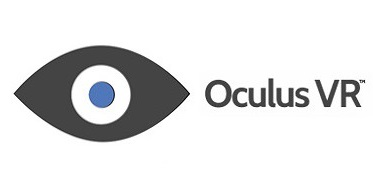
\includegraphics[width=0.25\textheight,left]{./images/oculus_logo.jpg}
        
\includegraphics[width=0.25\textheight,right]{./images/Unity_3D_logo.png}

  \end{titlepage}
\makeatother
%\end --------------------------------------------------------------------

%table des matières :
\setlength{\textheight}{26cm}
\setlength{\topmargin}{-2cm}

\tableofcontents


\newpage
\section*{Remerciements}
\par Tout d'abord nous tenons à remercier M. Lebrun pour nous avoir proposer le projet. Pour son suivi, la documentation et les conseils qu'il nous a fourni.
Pour nous avoir prêter l'oculuse VR pendant plusieurs semaines pour faire des tests.


\chapter{Introduction}
\par Le projet Oculus VR consiste en la réalisation d'un jeu à but pédagogique. Destiné à la promotion de l'école lors des journées portes ouvertes et des journées de l'étudiant en fin d'année 2015.
\par La réalisation du projet comprend l'utilisation de la technologie de réalité augmenté \''Oculus VR V2\'' détenu aujourd'hui par le groupe Facebook. Le modèle d'essaye appartient au laboratoire de recherche de l'ENSICAEN. Prêté pour le projet par Gilles Lebrun lors de nos tests.
\begin{figure}[h] 
	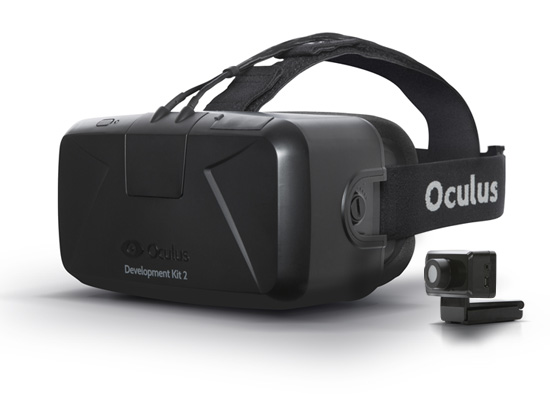
\includegraphics[scale=0.70]{./images/dk2-product.jpg}
	\caption{Casque Oculus VR kit de developpement version 2}
\end{figure}


\chapter{Contexte}
\par Aujourd'hui les jeux vidéos étant un média incontournable, beaucoup de société s'oriente vers l'utilisation de ceux-ci pour promouvoir, divertir, instruire le grand public. Notre projet ce situe entre le ludisme et la pédagogie et évidement, doit promouvoir en un sens, les compétences acquises lors de la formation à l'école.
\par Pour ce faire nous avons accès à une technologie remise au goût du jour il y a 3 ans, grâce à une campagne Kickstarter\footnote{Kickstarter : Plateform collaborative de participation en ligne à des projets divers.} : La réalité augmentée.

\section{Jeu}
\par Notre jeu consiste à réaliser un algorithme à l'aide de cubes de différents couleurs. Évidemment il ne s'agit pas de les placer dans n'importe quel ordre pour que cela fonctionne.\\
On a donc pour référence, des cubes de couleur dans une zone dédiée, qui nous indiquent quel résultat on doit obtenir. On aussi des emplacement labellisés qui permettent de se faire une idée du type de cube à déposer pour que cela fonctionne. 


\chapter{Réalisation}
\section{Outils}
\subsection{Choix du moteur}
\par Le choix du moteur\footnote{moteur de jeu : Logiciel permettant de réaliser des jeux vidéos grâce à une base logiciel conséquente, le code qu'on y ajoute et éventuellement une interface graphique et des scripts pré-existants.} est une partie important du projet. Même si avant même de commencer le projet nous avions déjà une idée du moteur que nous souhaitions utiliser, nous avons joué le jeu et essayer les deux logiciels. \`A savoir Blender Game Engine, un logiciel gratuit qui utilise python pour le rendu et Unity qui est un peu plus reconnu dans le monde professionnel mais payant. Unity prend en charge le JavaScript, le Boo et le C\# comme langage de programmation.

\par Comme nous sommes plus à l'aise avec le Java Unity marque un point avec le C\#, qui est facile à prendre en main quand on connait le Java. Ensuite lors de nos tests nous avons remarqué que l'interface de Blender est difficile à prendre en main. Elle nécessite de prendre en main un minimum de raccourcis clavier. Sans quoi les dizaines de boutons de l'interface sont un problème. Nous n'avons donc jamais produire un jeu en python avec Blender en une semaine de tests.
\par Par contre Unity est très facile à prendre en main. L'interface est assez agréable et simple d'utilisation.
\\Au final, voici la liste des avantages et inconvénients de chacun des deux logiciels :

  \begin{description}
  	\item \textbf{Blender Game Engine :}
  	\begin{itemize}
  		\item Interface difficile à prendre en main.
  		\item Reprendre le python pour programmer.
  		\item Pas d'intégration \''simple\'' de l'oculus.
  		\item Pas d'éditeur de script convivial.
  		\item Gratuit.
  		\item Beaucoup de tutoriels et d'aide sur internet.
  		\item Un mode pour la modélisation et un mode pour créer des jeux.
  	\end{itemize}
  	\item \textbf{Unity 3D :}
  		\begin{itemize}
  			\item Pas de mode dédié à la modélisation d'objets.
  			\item Payant.
  			\item MonoDevelop\footnote{MonoDevelop : IDE proposé par unity pour éditer les scripts qu'on attache au jeu.} peu pratique.
  			\item Kit d'intégration oculus développé pour Unity 3D.
  			\item Facile à prendre en main.
  			\item Possibilité de développer avec un langage objet (C\#).
  			\item Compatible avec Visual Studio.
  		\end{itemize}
  \end{description}
  
  \par Après s'être renseigner nous avons vu qu'il était possible de travailler à sur Unity sans payer (version d'évaluation). Comme le projet n'est pas utilisé à des fins commerciales, pas de soucis.
  \par Nous avons donc choisi Unity couplé au C\# pour les scripts. Nous détaillerons ce point juste après.
  
  \subsection{Le langage de programmation}
  \par Le langage de programmation ne nous été pas imposé. Donc nous nous sommes tournés rapidement vers le plus familier, le C\#. Un langage objet qui ressemble beaucoup au Java. Utilisé beaucoup pour développer des application pour Windows.
  \par Nous avons aussi testé le JavaScript mais pas le Boo. En récupérant des morceaux de codes sur internet (souvent disponible dans les 3 langages) on peut facilement porter un script d'un langage à un autre.
  Par contre on ne peut pas faire appel à un script JavaScript dans un script C\# par exemple. Donc il faut que le langage de programmation soit unifié.


\subsection{Environnement de développement}
\par Comme nous l'avons précisé plus tôt, Unity propose un environnement de développement (MonoDevelop). Il est sommaire mais plutôt efficace. Cependant il n'est pas parfaitement au point et laisse à désirer parfois.
Comme nous développons sous Windows, VisualStudio Community (pour la version gratuite) est disponible. Et il propose un pluging pour Unity ce qui fut une fort bonne nouvelle.
\par Ce pluging donne accès à des fonctionnalités comme l'attachement du script à Unity pour détecter les erreurs liés à la bibliothèque de Unity sans lancer le jeu. Une autocomplétion qui prend aussi bien en charge le C\# que la bibliothèque Unity, ce qui n'est pas le cas de MonoDevelop. Et un gestionnaire de version plus poussé que sur MonoDevelop mais qui laisse assez septique parfois tout de même.
Au final, pour la gestion de version, GitShell et les linges de commande étaient nettement plus efficace. Le dépôt GitHub est disponible \href{https://github.com/manumanmax/SeriousVR.git}{ici}.

\section{Développement}
\subsection{Prise en main}

\par Nous avons commencé par une longue phase de prise en main. D'abord de l'interface de Unity, ce qui fut assez rapide. Puis des scripts, ce qui prit beaucoup plus de temps.
Unity propose tout d'abord une classe MonoBehavior. Celle-ci implémente les méthodes classiques comme \''start\'' et \''update\'' qui sont respectivement lancées à l'instanciation de la classe et toute les frames\footnote{Frame: Anglissisme qui désigne une image générée par le jeu. Qui s'affiche entre 30 et 60 fois par seconde généralement.}. 
L'oculus VR nous a aussi pris beaucoup de temps. C'est une technologie assez capricieuse car il faut faire attention à la compatibilité des pilotes. Que l'application dédiée soit installée sur un système d'exploitation sans trop de virus. Il ne faut pas de résolution d'affichage ou propriété d'affichage un peu exotiques. Sinon même un simple jeu de démonstration ne pourra pas se lancer correctement.
Et même une fois avec testé une application on ne peut pas être certain que cela dur.
\par Lors de nos tests nous avons quand même pu lancer la démonstration \''Toscany\'' offerte dans l'API Oculus. Nous avons pu remarquer que le système requière un ordinateur avec une carte graphique assez puissante (Gefore GTX récent ou équivalent, parfaitement suffisant). Et on se laisse prendre au jeu de la perspective facilement. Attention tout de même à ne pas en abuser car des effets de nausées peuvent être ressentis rapidement. 
Quand bien même, une fois la caméra intégrée à une scène Unity et l'exportation faite. Nous avons pu voir qu'il était simple d'utiliser l'Oculus avec Unity 3D.
\subsection{Sprints}
\par Nous avons tenté de faire un développement régulier mais ce ne fut pas évident avec les cours en parallèle du projet. Le développement c'est plus fait sous forme de sprints.
D'abord pour nos différents tests, puis pour la conception des différentes briques du jeu final.
Chaque sprint était dédié à une fonctionnalité et ne durait pas plus de quelques heures. Ce qui, au final, répartissait bien la charge de travail, permettait d'implémenter des composants atomique et de mieux apprécier  l'avancement du projet.

\subsection{Répartition des tâches}
\par Nous nous sommes réparti les test, Benjamin plutôt le côté modélisation et affichage de labels, Emmanuel plutôt le côté algorithmique et intégration des scripts.
\par Le dépôt GitHub était partagé donc nous travaillions sur des branches différentes. Au final nous n'avons donc pas défini d'intégrateur.
\par Emmanuel c'est chargé de la relation avec M. Lebrun, des tests de l'oculus et de la mise en place du niveau de la version finale.

\newpage

\chapter{Résultats}
\par Le jeu à nécessité plusieurs points de concentration. D'abord la réalisation d'une scène qui regroupe tous les éléments nécessaires à la réalisation d'un algorithme. Une scène peu être inter-changée et on peut sauvegarder des paramètres de la scène précédente si nécessaire. Dans notre cas, une seule scène est utilisée, ce qui facilite un peu les choses. 
\par Elle contient des \''GameObject\'', types primitifs de Unity 3D auquel on peut attacher des composants. Plus de détails seront données dans la partie \textit{objet} qui suit.
	\section{Scène}
	\par Lorsqu'on lance Unity3D la dernière scène est chargée si on travaillait sur une scène. Dans le cas contraire elle est automatiquement crée et appelée level1. Non n'avions donc rien à faire pour créer la scène et déjà nous pouvions la lancer.
	Pour la remplir, on peut utiliser les objets primitifs de Unity3D comme des cubes, plans ou sphères (assez limité). Fort heureusement on peut importer des modèles 3D d'autres éditeurs, comme Blender par exemple. C'est très simple, on ouvre le dossier et un cliquer glisser suffit pour l'ajouter dans le projet.
	\par L'interface graphique dans la partie qui représente la scène permet de se déplacer dans le monde 3D. De déplacer les objets et de modifier leur taille.
	Sur la partie droite on a accès au propriétés de l'objet sur lequel on travail.
	\begin{figure}[h]
	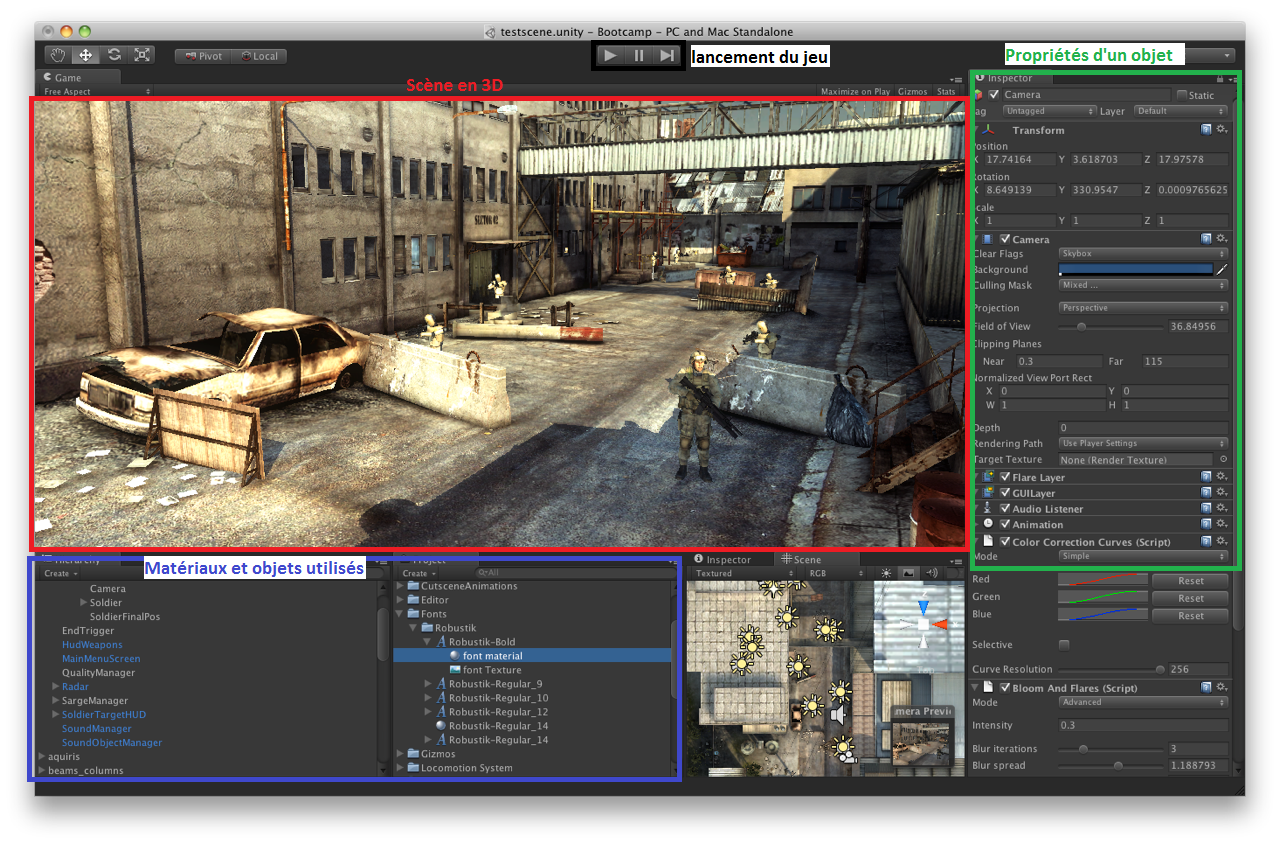
\includegraphics[scale=0.35]{./images/unity-3D_interface.png}
	\caption{Interface graphique de Unity3D}
	\end{figure}
	
	\newpage
	\subsection{Objets}
	\par Sur la scène nous venons de dire qu'il y a des \textit{GameObject}, et ils sont très importants. En effet, même un objet invisible dans le jeu peut être très utile.
	Les objets ou gameObjects on la particularité se voir greffer un certain nombre de composants, primitif à Unity3D ou non, qui eux même peuvent être modifiés. Voir \hyperlink{prefabTarget}{ici} pour aller encore plus loin avec les prefabs.

	\par Dans le projet nous avons des plans pour faire les murs et les écrans. Ils ont un matériaux, qui lui possède une texture\footnote{Texture : Image sur laquelle les rayons lumineux vont se projeter}. Les plateformes, elles, sont brutes (sans matériaux) mais comme tous les objets visibles à l'écran elles possède un \textit{meshRenderer} qui leur permet de renvoyer les rayons lumineux. D'ailleurs c'est pour cette même raison que la caméra n'a pas de MeshRenderer. C'est aussi le cas pour l'objet \textit{Algorithm} qui lui ne possède qu'un script. Nous en parlerons dans une \hyperlink{prefabTarget}{section} dédiée.

	\subsection{Matériaux}
	\par Les matériaux sont une primitive de Unity3D et si nous avons décidé d'en parler c'est que dans la section qui suit, ils vont servir. Notamment à changer les cubes de couleur.\\
	C'est donc comme son nom l'indique, un composant\footnote{Composant : Nous appellerons dorénavant les primitives et script qu'on greffe à un GameObject : un composant, traduit de component dans Unity3D} indique comment la lumière va se refléter. Ils font intervenir des shaders que nous n'allons pas aborder dans se rapport.\\
	Un matériaux à une couleur, un type de réfraction de la lumière (diffus ou/et spéculaire généralement) et une texture. La texture et la couleur son complémentaires. C'est-à-dire qu'on peut colorer une texture sans la modifier, juste par additivité avec la couleur du matériaux.
	\begin{figure}[h]
	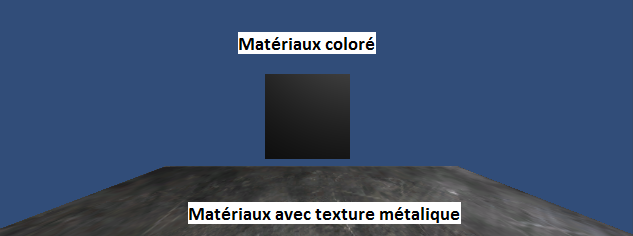
\includegraphics[scale=0.50]{./images/materiaux.png}
	\caption{Colorer avec ou sans texture}
	\end{figure}
	\par Exactement la même scène mais cette fois avec de la couleur dans le matériaux en plus de la texture. On obtient un effet cuivré.
	\begin{figure}[h]
	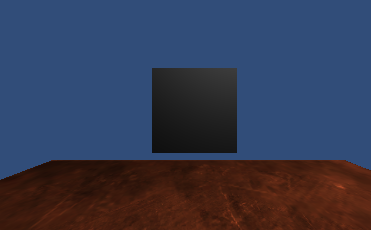
\includegraphics[scale=0.40]{./images/materiaux_cuivre.png}
	\caption{Modification de la composante MainColor du matériaux}
	\end{figure}
	\par Dans cette exemple nous utilisons l'interface graphique pour obtenir ce résultat. Cela prend quelques minutes tout au plus. La bonne nouvelle est qu'il en va de même dans un script. Cela nécessite quelques minutes pour obtenir le même résultat. Et cela nous servira grandement pour colorier nos cubes.
	\section{Scripts}
	\hypertarget{scriptTarget}{Les} Scripts
	\subsection{Pour la caméra}
	\subsection{Pour l'algorithme}
	\subsection{Pour stocker les objets des récepteurs}
	\section{Prefabs}
	\hypertarget{prefabTarget}{Les} Prefabs
	\subsection{Boucle}
	\subsection{cubes}

\chapter{Difficultés}
rigidbody
\chapter{Apports personnels}

\chapter{Glossaire}

\chapter{Annexes}

\begin{figure}[h]
	
\includegraphics[scale=0.70]{./images/LogoEnsicaenSansTexte.jpg}
	\caption{JDialog permettant le réglage d'une LED 4 couleurs}
\end{figure}
\listoffigures
\end {document}
